\chapter{Multichannel Denoising and Deconvolution on the Sphere}
\label{ch_multichannel}

\section{Introduction}
 
This chapter describes how to remove Poisson noise while deconvolving the effect of the PSF, and presents an multichannel extension of the restoration process.
Indeed, some  instruments  such as FERMI-LAT  produce 2D-1D  data where the two first dimensions are spatial (longitude and latitude) and the third dimension is either the time or the energy. 
We present here  a multichannel sparse representation for Poisson data combining the MS-VSTS with a spherical 2D-1D wavelet-based deconvolution algorithm. 
This multiscale representation is used in a wavelet-regularized Richardson-Lucy deconvolution algorithm to remove the effect of the PSF. This method has the advantage to take into account 
the strong energy dependence of PSF, and the recovering of the spectral information of point sources.

Section 2 proposes a multichannel representation of spherical Poisson data based on the MS-VSTS and a 2D-1D spherical wavelet transform. Section 3 applies the multichannel MS-VSTS to Poisson denoising. Section 4 applies the multichannel MS-VSTS to Poisson deconvolution.

Experiments are based on simulated Fermi HEALPix cubes ($nside=256$) with 14 energy bands between 50 MeV and 50 GeV.
 
\section{Sparse Representation for Multichannel Spherical Data with Poisson Noise}

\subsection{Fast Undecimated 2D-1D Wavelet Decomposition/Reconstruction on the Sphere}

We propose a denoising method for 2D - 1D data on the sphere, where the two first dimensions are spatial (longitude and latitude) and the third dimension is either the time or the energy. We need to analyze the data with a non-isotropic wavelet, where the time or energy scale is not connected to the spatial scale. We use a spherical extension of the Fast Undecimated 2D-1D Wavelet Transform proposed in \citet{Starck09:fermi3d}.

%In order to have a fast algorithm for discrete data, we use wavelet functions associated to filter banks. 

For a given data set $D(k_{\theta},k_{\varphi},k_{t})$ ($k_{\theta}$ and $k_{\varphi}$ are spatial index and $k_{z}$ a time (or energy) index), the 2D-1D decomposition consists in applying first a IUWT on the sphere for each frame $k_t$. Using the spherical IUWT, we have the reconstruction formula:
%Hence, our wavelet decomposition consists in applying first a IUWT on the sphere for each frame $k_z$. Using the spherical IUWT, we have the reconstruction formula:
\begin{equation}
\label{reconstiuwt}
D[k_{\theta},k_{\varphi},k_{t}]  = a_{J_1}[k_{\theta},k_{\varphi}] + \sum_{j_1=1}^{J1}w_{j_1}[k_{\theta},k_{\varphi},k_{t}], \forall k_{t}
\end{equation}
where $J_1$ is the number of spatial scales. To have lighter notations, we replace the two spatial indexes by a single index $k_r$ which corresponds to the pixel index:
\begin{equation}
\label{reconstiuwtpix}
D[k_{r},k_{t}]  = a_{J_1}[k_{r}] + \sum_{j_1=1}^{J1}w_{j_1}[k_{r},k_{t}], \forall k_{t}
\end{equation}
Then, for each spatial location $k_r$ and for each 2D wavelet scale $j_1$, we apply a 1D wavelet transform along $t$ on the spatial wavelet coefficients $w_{j_1}[k_r,k_t]$ such that
\begin{equation}
\label{decompwavj1}
w_{j_1}[k_r,k_t] = w_{j_1,J_2} [k_r,k_t] + \sum_{j_2=1}^{J_2}w_{j_1,j_2}[k_r,k_t], \forall(k_r,k_t)
\end{equation}
where $j_2$ is the number of scales along $t$.The same processing is also applied on the coarse spatial scale $a_{J_1}[k_r,k_t]$ and we have
\begin{equation}
\label{decompaj}
a_{J_1}[k_r,k_t] = a_{J_1,J_2} [k_r,k_t] + \sum_{j_2=1}^{J_2} w_{J_1,j_2}[k_r,k_t], \forall(k_r,k_t)
\end{equation}
Hence, we have a 2D-1D spherical undecimated wavelet representation of the input data $D$:
\begin{equation}
\label{decomp2d1d}
D[k_r,k_t] = a_{J_1,J_2}[k_r,k_t] + \sum_{j_1=1}^{J_1}w_{j_1,J_2} [k_r,k_t] + \sum_{j_2=1}^{J_2} w_{J_1,j_2} [k_r,k_t] + \sum_{j_1=1}^{J_1}\sum_{j_2=1}^{J_2} w_{j_1,j_2} [k_r,k_t]
\end{equation}
From this expression, we distinguish four kinds of coefficients:
\begin{itemize}
  \item Detail-Detail coefficients ($j_1 \leqslant J_1$ and $j_2 \leqslant J_2$):
  \begin{equation}
  \label{detaildetail}
w_{j_1,j_2}[k_r,k_t] = (\delta - \bar{h}_{1D}) \star (\bar{h}_{1D}^{(j_2-1)} \star a_{j_1-1}[k_r,\cdot]
- h_{1D}^{(j_2-1)} \star a_{j_1}[k_r,\cdot])
  \end{equation}
  \item Approximation-Detail coefficients ($j_1 = J_1$ and $j_2 \leqslant J_2$):
\begin{equation}
\label{approxdetail}
w_{J_1,j_2}[k_r,k_t] = h_{1D}^{(j_2-1)} \star a_{J_1}[k_r,\cdot] - h_{1D}^{(j_2)} \star a_{J_1}[k_r,\cdot]
\end{equation}
  \item Detail-Approximation coefficients ($j_1 \leqslant J_1$ and $j_2 = J_2$):
\begin{equation}
\label{detailapprox}
w_{j_1,J_2}[k_r,k_t] = h_{1D}^{(J_2)} \star a_{j_1-1}[k_r,\cdot] - h_{1D}^{(J_2)} \star a_{j_1}[k_r,\cdot]
\end{equation}
  \item Approximation-Approximation coefficients ($j_1 = J_1$ and $j_2 = J_2$):
\begin{equation}
\label{approxapprox}
a_{J_1,J_2}[k_r,k_t] = h_{1D}^{(J_2)} \star a_{J_1}[k_r,\cdot]
\end{equation}
\end{itemize}


\subsection{Poisson Noise}

\subsubsection{The Multi-Scale Variance Stabilizing Transform on the Sphere (MS-VSTS)}

\citet{Schmitt} proposed a multiscale decomposition on the sphere adapted for spherical data with Poisson noise, called Multi-Scale Variance Stabilizing Transform on the Sphere (MS-VSTS) (see previous chapters). This method consists in mixing a multi-scale transform (for instance the Isotropic Undecimated Wavelet Transform on the Sphere) with a variance stabilizing transform (VST), in order to have "Gaussianized" multiscale coefficients.

The recursive scheme of the MS-VSTS with IUWT is:
This section describes the MS-VSTS + IUWT, which is a combination of a square-root VST with the IUWT. The recursive scheme is:
\begin{equation}
\label{mc_eq27}
\begin{split}
&\text{IUWT}\left\{\begin{array}{ccc}a_j  & = &  h_{j-1} \ast a_{j-1}  \\d_j  & = & a_{j-1}  - a_j  \end{array}\right. \\
 \Longrightarrow & \begin{split}\text{MS-VSTS} \\  \text{+ IUWT} \end{split}\left\{\begin{array}{ccc}a_j  & = &  h_{j-1} \ast a_{j-1} \\d_j  & = & T_{j-1}(a_{j-1}) - T_j(a_j) \end{array}\right. .
\end{split}
\end{equation}
where $T_j$ is the VST operator at scale $j$:
\begin{equation}
\label{mc_eq28}
T_j(a_j) = b^{(j)} \mathrm{sign}(a_j+c^{(j)})\sqrt{|a_j + c^{(j)}|} .
\end{equation}
It has been shown that the detail coefficients $d_j$ issued from locally homogeneous parts of the signal follow asymptotically a central normal distribution with an intensity-independant variance which relies solely on the filter $h$ and the current scale for a given filter $h$. Consequently, the stabilized variances and the constants $b^{(j)}$ and $c^{(j)}$ can all be pre-computed \cite{Schmitt}.


\subsubsection{Multichannel MS-VSTS}

%To perform a Poisson denoising, we have to plug the MS-VST into the spherical 2D-1D undecimated wavelet transform.


We propose a multichannel extension of the MS-VSTS method. We plug the VST into the spherical 2D-1D undecimated wavelet transform.
Again, we distinguish four kinds of coefficients that take the following forms:
\begin{itemize}
  \item Detail-Detail coefficients ($j_1 \leqslant J_1$ and $j_2 \leqslant J_2$):
  \begin{equation}
  \label{detaildetailmsvst}
w_{j_1,j_2}[k_r,k_t] = (\delta - \bar{h}_{1D}) \star ( T_{j_1-1,j_2-1} [\bar{h}_{1D}^{(j_2-1)} \star a_{j_1-1}[k_r,\cdot] ] 
- T_{j_1,j_2-1}[h_{1D}^{(j_2-1)} \star a_{j_1}[k_r,\cdot]])
  \end{equation}
  \item Approximation-Detail coefficients ($j_1 = J_1$ and $j_2 \leqslant J_2$):
\begin{equation}
\label{approxdetailmsvst}
w_{J_1,j_2}[k_r,k_t] = T_{J_1,j_2-1}[h_{1D}^{(j_2-1)} \star a_{J_1}[k_r,\cdot]] - T_{J_1,j_2}[h_{1D}^{(j_2)} \star a_{J_1}[k_r,\cdot]]
\end{equation}
  \item Detail-Approximation coefficients ($j_1 \leqslant J_1$ and $j_2 = J_2$):
\begin{equation}
\label{detailapproxmsvst}
w_{j_1,J_2}[k_r,k_t] = T_{j_1-1,J_2} [h_{1D}^{(J_2)} \star a_{j_1-1}[k_r,\cdot]] - T_{j_1,J_2} [h_{1D}^{(J_2)} \star a_{j_1}[k_r,\cdot]]
\end{equation}
  \item Approximation-Approximation coefficients ($j_1 = J_1$ and $j_2 = J_2$):
\begin{equation}
\label{approxapproxmsvst}
a_{J_1,J_2}[k_r,k_t] = h_{1D}^{(J_2)} \star a_{J_1}[k_r,\cdot]
\end{equation}
\end{itemize}

Hence, all 2D-1D wavelet coefficients $w_{j_1,j_2}$ are now stabilized, and the noise on all these wavelet coefficients is Gaussian with known scale-dependent variance that depends solely on $h$. %Denoising is however not straightforward because there is no explicit reconstruction formula available because of the form of the stabilization equations above. Formally, the stabilizing operators $T_{j_1,j_2}$ and the convolution operators along the spatial and temporal dimensions do not commute, even though the filter bank satisfies the exact reconstruction formula. To circumvent this difficulty, we propose to solve this reconstruction problem by using an iterative reconstruction scheme.

%exemple : transfo d'un dirac

\section{Application to Multichannel Denoising}

\subsection{Gaussian Case}


As the spherical 2D-1D undecimated wavelet transform described before is fully linear, a Gaussian noise remains Gaussian after transformation. Therefore, all thresholding strategies which have been developed for wavelet Gaussian denoising are still valid with the spherical 2D-1D wavelet transform. Denoting TH the thresholding operator, the denoised cube in the case of additive white Gaussian noise is obtained by:
\begin{equation}
\label{denoisegaussmc}
\tilde{D}[k_r,k_t] = a_{J_1,J_2}[k_r,k_t] + \sum_{j_1=1}^{J_1}\text{TH}(w_{j_1,J_2} [k_r,k_t]) + \sum_{j_2=1}^{J_2} \text{TH}(w_{J_1,j_2} [k_r,k_t]) + \sum_{j_1=1}^{J_1}\sum_{j_2=1}^{J_2} \text{TH}(w_{j_1,j_2} [k_r,k_t])
\end{equation}
A typical choice of TH is the hard thresholding operator, i.e.:
\begin{equation}
\label{hardthresh}
\text{TH}(x) = \left \{ \begin{array}{cc}0 & if |x| < \tau \\x & if |x| \geqslant \tau \end{array}\right.
\end{equation}
The threshold $\tau$ is generally chosen between $3$ and $5$ times the noise standard deviation.


\subsection{Poisson Case}

%Hence, all 2D-1D wavelet coefficients $w_{j_1,j_2}$ are now stabilized, and the noise on all these wavelet coefficients is Gaussian with known scale-dependent variance that depends solely on $h$. Denoising is however not straightforward because there is no explicit reconstruction formula available because of the form of the stabilization equations above. Formally, the stabilizing operators $T_{j_1,j_2}$ and the convolution operators along the spatial and temporal dimensions do not commute, even though the filter bank satisfies the exact reconstruction formula. To circumvent this difficulty, we propose to solve this reconstruction problem by using an iterative reconstruction scheme.

We perform a MS-VSTS transform on the data. As the noise on the stabilized coefficients is Gaussian, and without loss of generality, we let its standard deviation equal to $1$, we consider that a wavelet coefficient $w_{j_1,j_2}[k_r,k_t]$ is significant, i.e., not due to noise, if its absolute value is larger than a critical threshold $\tau$, where $\tau$ is typically between $3$ and $5$. Denoising is however not straightforward because there is no explicit reconstruction formula available because of the form of the stabilization equations above. Formally, the stabilizing operators $T_{j_1,j_2}$ and the convolution operators along the spatial and temporal dimensions do not commute, even though the filter bank satisfies the exact reconstruction formula. To circumvent this difficulty, we propose to solve this reconstruction problem by using an iterative reconstruction scheme.

\subsection{Iterative Reconstruction}


We define a multiresolution support which is obtained by detecting at each scale the significant coefficients. The multiresolution support for $j_1 \leqslant J_1$ and $j_2 \leqslant J_2$ is defined as:
\begin{equation}
\label{supportmr}
\mathcal{M}_{j_1,j_2}[k_r,k_t] = \left\{\begin{array}{cc}1 & \text{if } w_{j_1,j_2}[k_r,k_t] \text{ is significant} \\0 & \text{otherwise} \end{array}\right.
\end{equation}

We denote $\mathcal{W}$ the spherical 2D-1D undecimated wavelet transform described above, and $\mathcal{R}$ the inverse wavelet transform. We want our solution $X$ to preserve the significant structures of the original data by reproducing exactly the same coefficients as the wavelet coefficients of the input data $Y$, but only at scales and positions where significant signal has been detected. At other scales and positions, we want the smoothest solution with the lowest budget in terms of wavelet coefficients. Furthermore, as Poisson intensity functions are positive by nature, a positivity constraint is imposed on the solution. It is clear that there are many solutions satisfying the positivity and multiresolution support consistency requirements, e.g. $Y$ itself. Thus, our reconstruction problem based solely on these constraints is an ill-posed inverse problem that must be regularized. Typically, the solution in which we are interested must be sparse by involving the lowest budget of wavelet coefficients. Therefore our reconstruction is formulated as a constrained sparsity-promoting minimization problem that can be written as follows
\begin{equation}
\label{minpoisson}
\min_{\mathbf{X}} \| \mathcal{W} \mathbf{X} \|_1 \text{ subject to } \left\{\begin{array}{c}\mathcal{M} \mathcal{W} \mathbf{X} = \mathcal{M} \mathcal{W} \mathbf{Y} \\ \mathbf{X} \geqslant 0 \end{array}\right.
\end{equation}
where $\|\cdot\|$ is the $l_1$-norm playing the role of regularization and is well known to promote sparsity \citep{Donoho2004b}. This problem can be solved efficiently using the hybrid steepest descent algorithm \citep{wave:yamada01,starck:zhang07}, and requires about $10$ iterations in practice. Transposed into our context, its main steps can be summarized as follows:

\begin{algorithm}[!h]
%\caption{MS-VSTS + IUWT Denoising}
\label{mc_alg2}
\begin{algorithmic}[1]
\REQUIRE $\quad$ Input noisy data $\mathbf{Y}$, a low-pass filter $h$, multiresolution support $\mathcal{M}$ from the detection step, number of iterations $N_{\max}$ \\
%\underline{\emph{\textbf{Detection}}} \\
\STATE Initialize $\mathbf{X}^{(0)} = \mathcal{M} \mathcal{W} \mathbf{Y} = \mathcal{M}w_{Y}$,
\FOR{$n=1$ to $N_{\max}$}
\STATE $\tilde{d} = \mathcal{M}w_Y + (1-\mathcal{M})\mathcal{W}X^{(n-1)}$,
\STATE $\mathbf{X}^{(n)} = P_{+}(\mathcal{R}\text{ST}_{\beta_n}[\tilde{d}])$,
\STATE Update the step $\beta_n = (N_{\max} - n)/(N_{\max} - 1)$
\ENDFOR

\end{algorithmic}
\end{algorithm}
where $P_+$ is the projector onto the positive orthant, i.e. $P_+(x) = max(x,0)$, $\text{ST}_{\beta_n}$ is the soft-thresholding operator with threshold $\beta_n$, i.e. $\text{ST}_{\beta_n}[x] = x-\beta_n\text{sign}(x)$ if $|x| \geqslant \beta_n$, and $0$ otherwise.

The final spherical MS-VSTS 2D-1D wavelet denoising algorithm is the following:

\begin{algorithm}[!h]
%\caption{MS-VSTS + IUWT Denoising}
\label{mc_alg1}
\begin{algorithmic}[1]
\REQUIRE $\quad$ Input noisy data $\mathbf{Y}$, a low-pass filter $h$, threshold level $\tau$ \\
%\underline{\emph{\textbf{Detection}}} \\
\STATE \emph{Spherical 2D-1D MS-VST:} Apply the spherical 2D-1D-MS-VST to the data using (\ref{detaildetailmsvst})-(\ref{approxapproxmsvst}).
\STATE \emph{Detection:} Detect the significant wavelet coefficients that are above $\tau$, and compute the multiresolution support $\mathcal{M}$.
\STATE \emph{Reconstruction:} Reconstruct the denoised data using the algorithm above.

\end{algorithmic}
\end{algorithm}

\subsection{Experiments}

%The algorithm has been applied on our simulated Fermi data set, with 14 energy bands between 50 MeV and 50 GeV. Figure \ref{denoisingmulti1} shows the result of the algorithm on 5 energy bands. %On Figure \ref{denoisingmulti2}, we compare the result of the multichannel MS-VSTS with a monochannel MS-VSTS on the data integrated along the energy axis. 
The algorithm has been applied on our simulated Fermi data set, with 7 energy bands between 50 MeV and 1.58 GeV. Figures \ref{denoisingmulti1} and \ref{denoisingmulti2} shows the result of the algorithm on 2 energy bands.
The multichannel MS-VSTS provides a performant denoising on each energy band and enables us to get the spectral information for each spatial position (Figure \ref{powspec}).

\begin{figure}
\begin{center}
%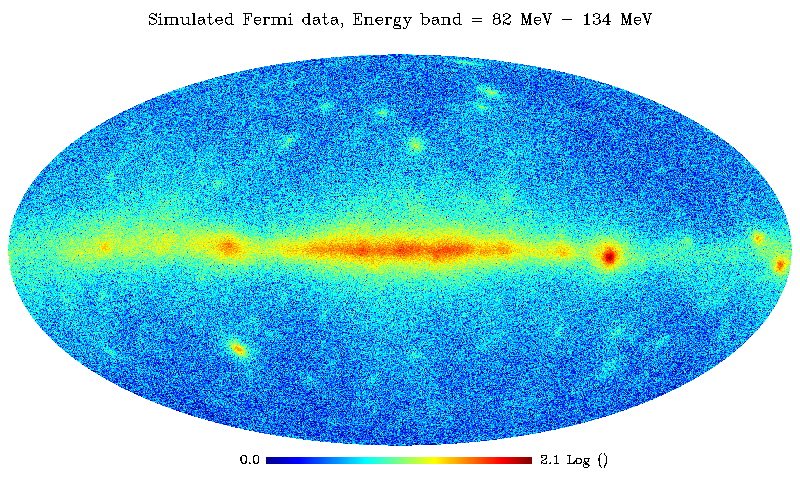
\includegraphics[width=2.9in]{data1.png} \hfill
%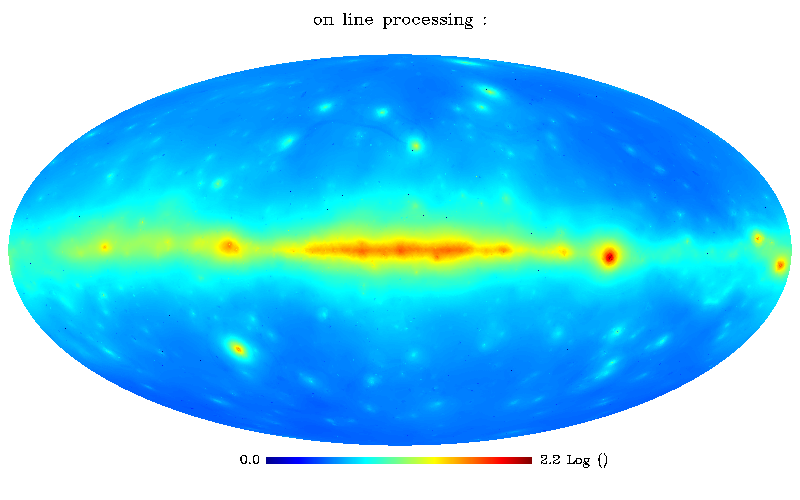
\includegraphics[width=2.9in]{sol1.png} \hfill
%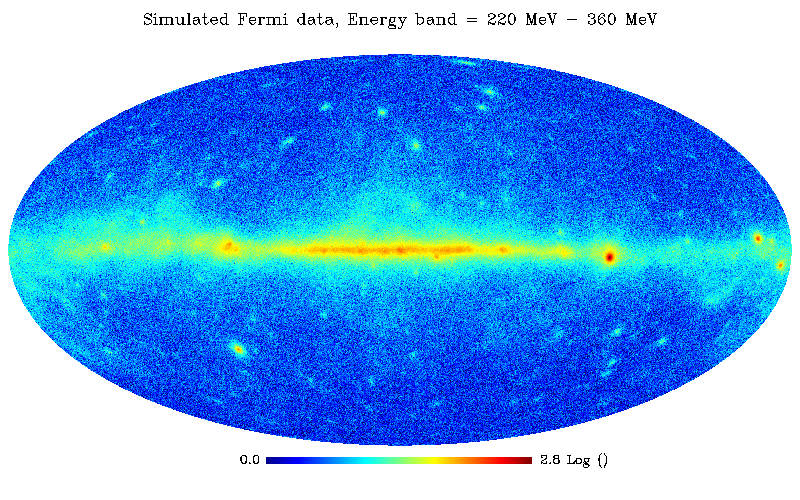
\includegraphics[width=3.8in]{data3.png} \hfill
%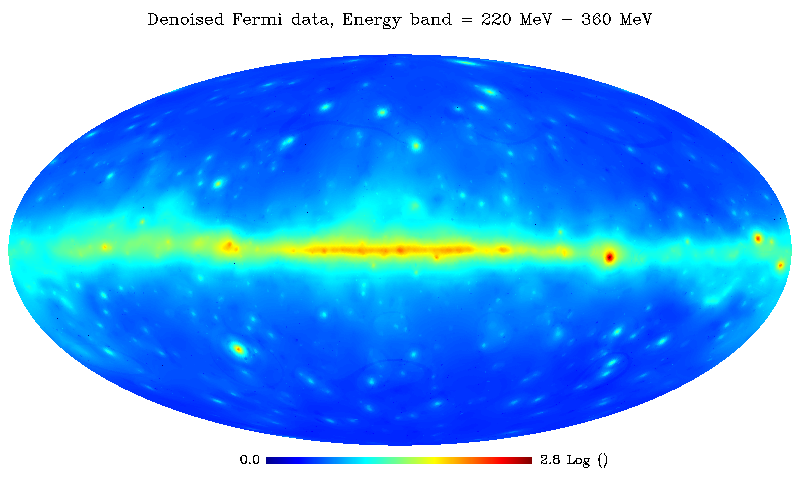
\includegraphics[width=3.8in]{sol3.png} \hfill
%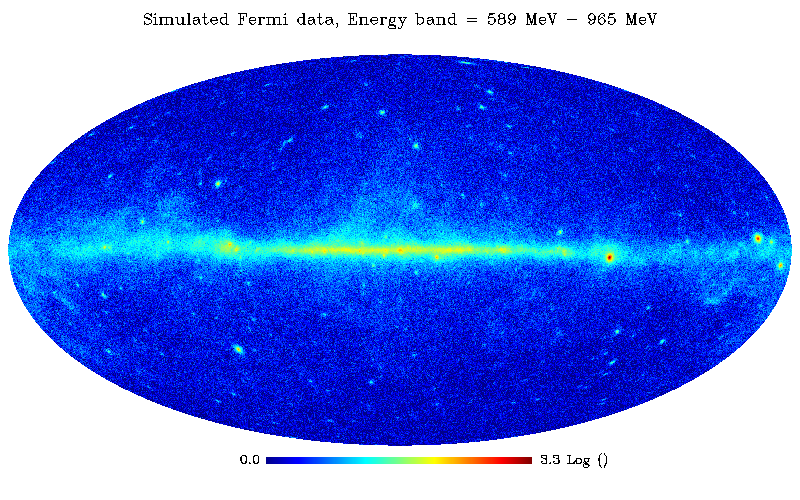
\includegraphics[width=3.8in]{data5.png} \hfill
%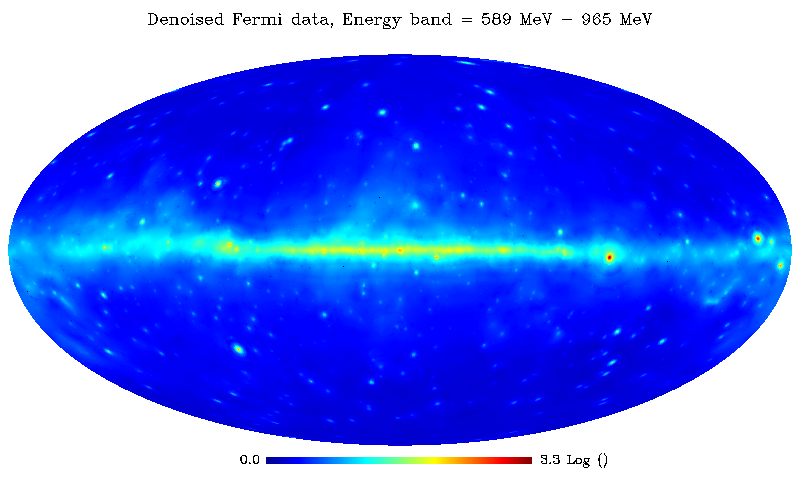
\includegraphics[width=3.8in]{sol5.png} \hfill
%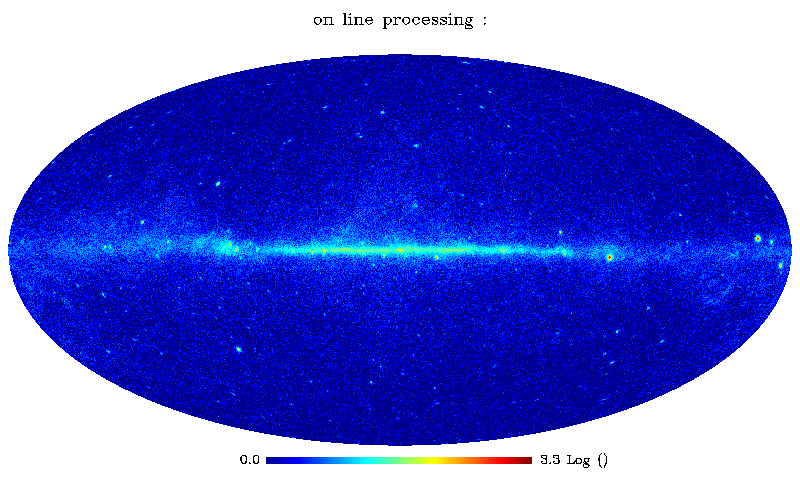
\includegraphics[width=3in]{data7.png} \hfill
%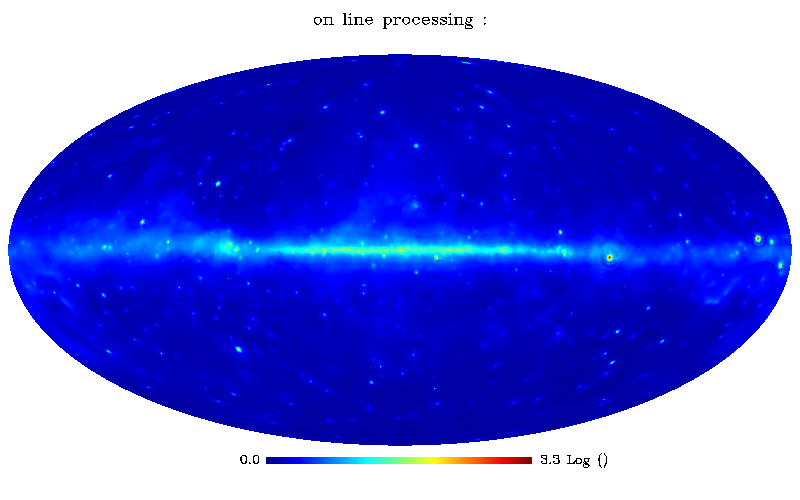
\includegraphics[width=3in]{sol7.png} \hfill
%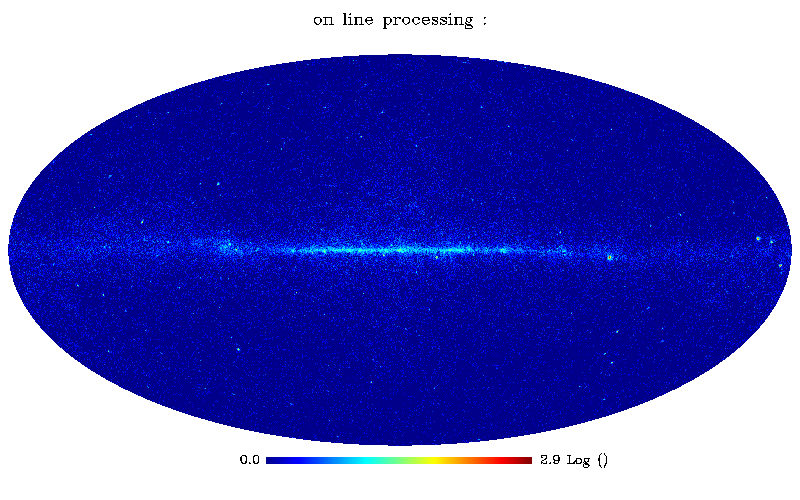
\includegraphics[width=2.9in]{data9.png} \hfill
%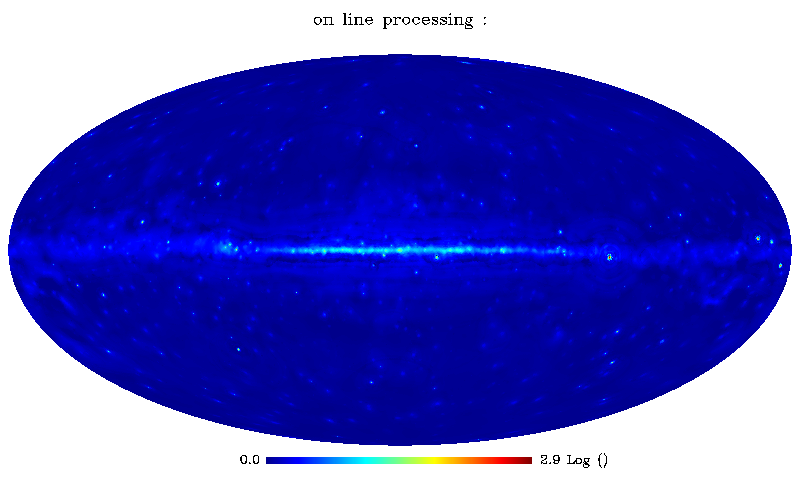
\includegraphics[width=2.9in]{sol9.png} \hfill
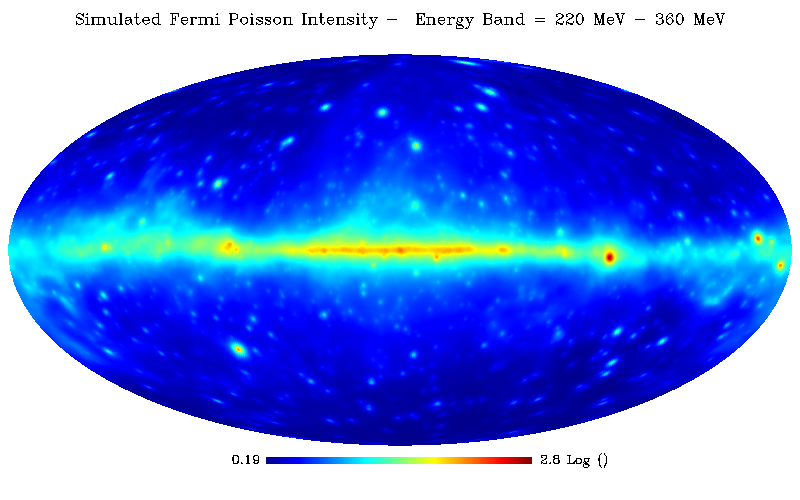
\includegraphics[width=3.8in]{plot_mc_intensityband3.png} \hfill
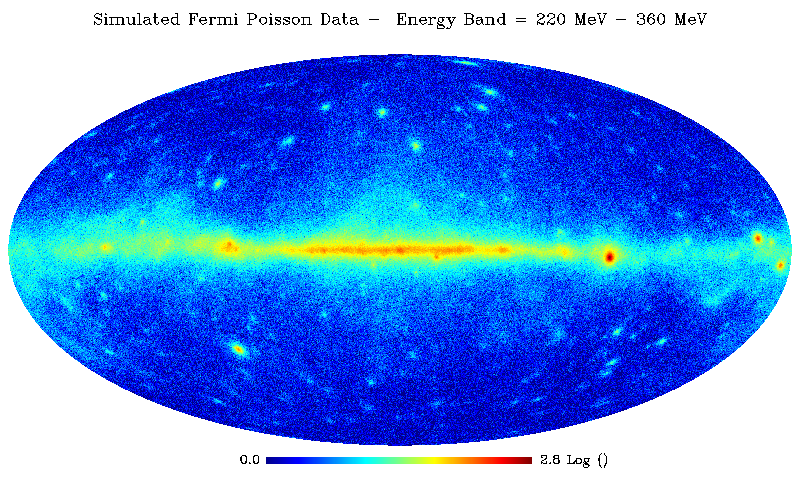
\includegraphics[width=3.8in]{plot_mc_simupoissonband3.png} \hfill
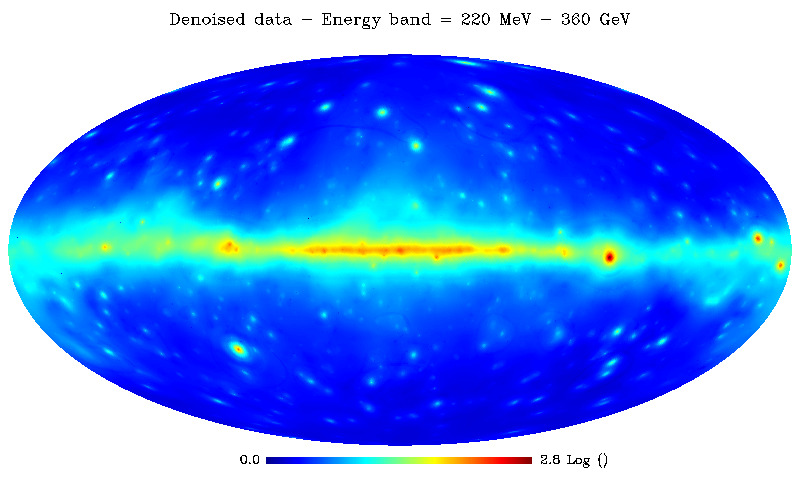
\includegraphics[width=3.8in]{plot_mc_simudenoisedband3.png} \hfill
\caption{Result of the multichannel Poisson denoising algorithm on simulated Fermi data on energy band 220 MeV - 360 MeV (\emph{Top:} Simulated intensity skymap. \emph{Middle:} Simulated noisy skymap. \emph{Bottom:} denoised skymap).
%Result of the multichannel Poisson denoising algorithm on simulated Fermi data on two different energy bands (Top : noisy skymap. Bottom : denoised skymap).
%Energy bands: 220 MeV - 360 MeV, 589 MeV - 965 MeV.
%Energy bands: 82 MeV - 134 MeV, 220 MeV - 360 MeV, 589 MeV - 965 MeV, 1.58 GeV - 2.59 GeV, 4.24 GeV - 69.5 GeV.
Pictures are in logarithmic scale.
}
\label{denoisingmulti1}
\end{center}
\end{figure}

\begin{figure}
\begin{center}
%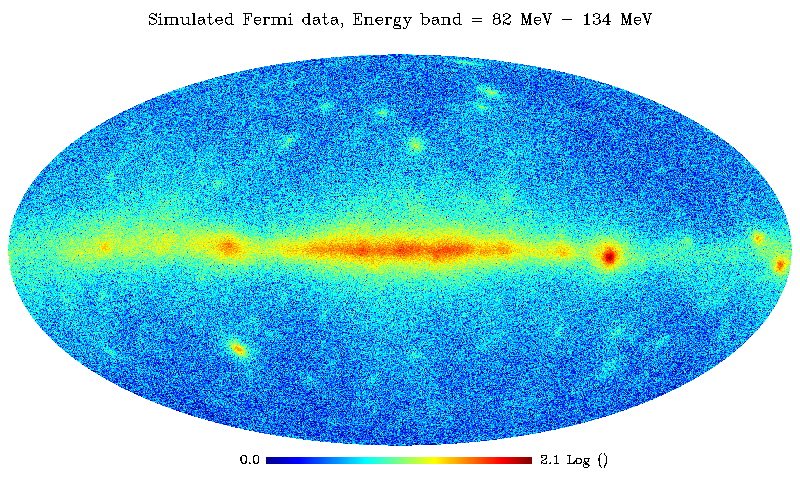
\includegraphics[width=2.9in]{data1.png} \hfill
%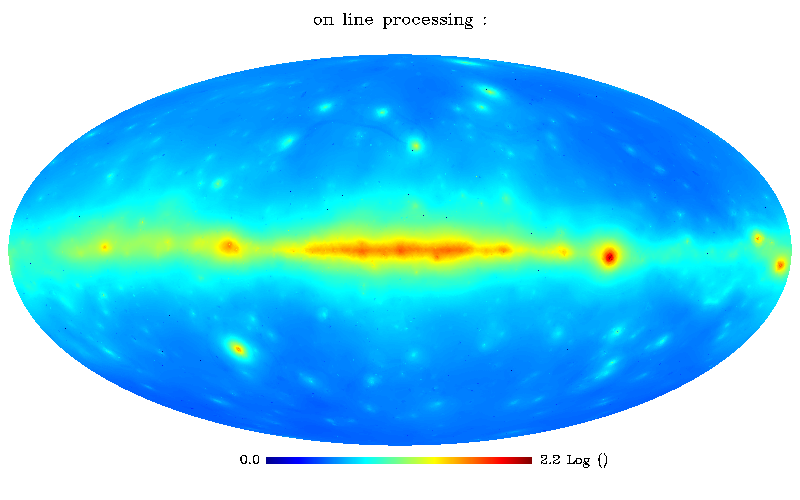
\includegraphics[width=2.9in]{sol1.png} \hfill
%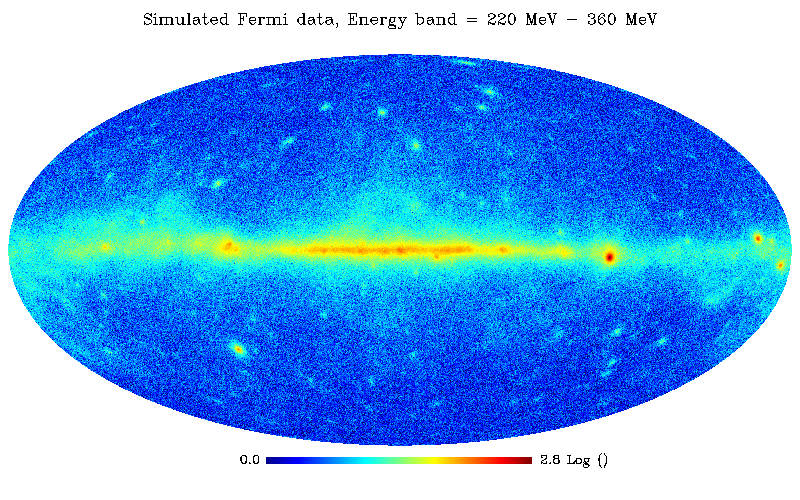
\includegraphics[width=3.8in]{data3.png} \hfill
%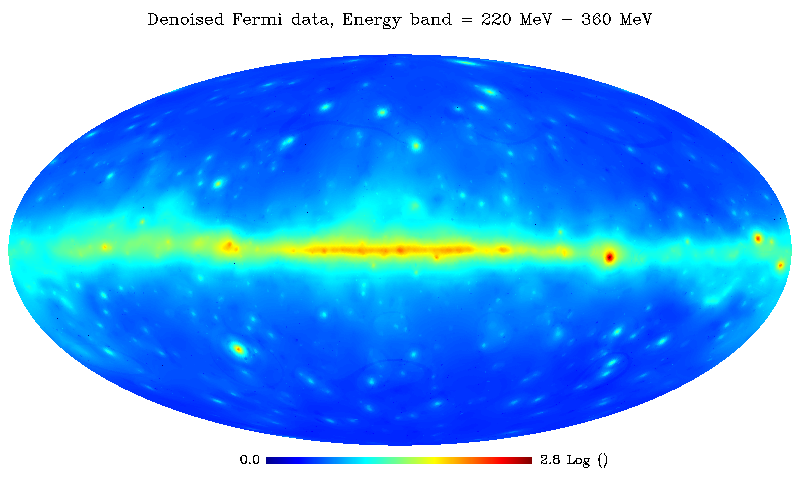
\includegraphics[width=3.8in]{sol3.png} \hfill
%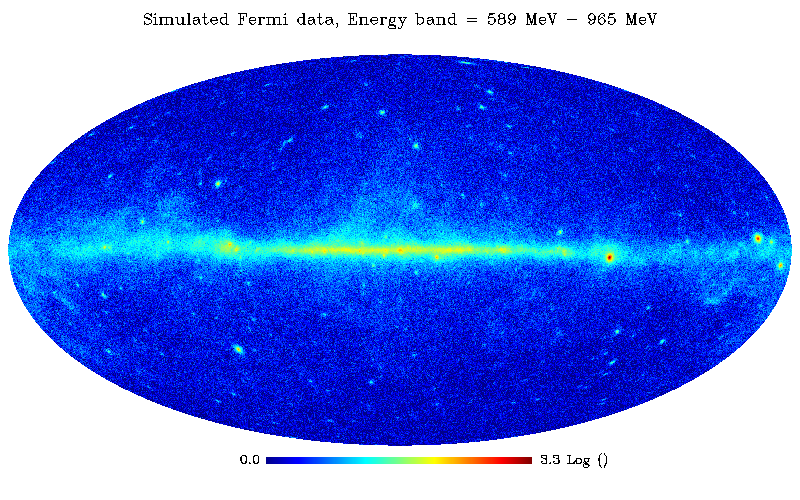
\includegraphics[width=3.8in]{data5.png} \hfill
%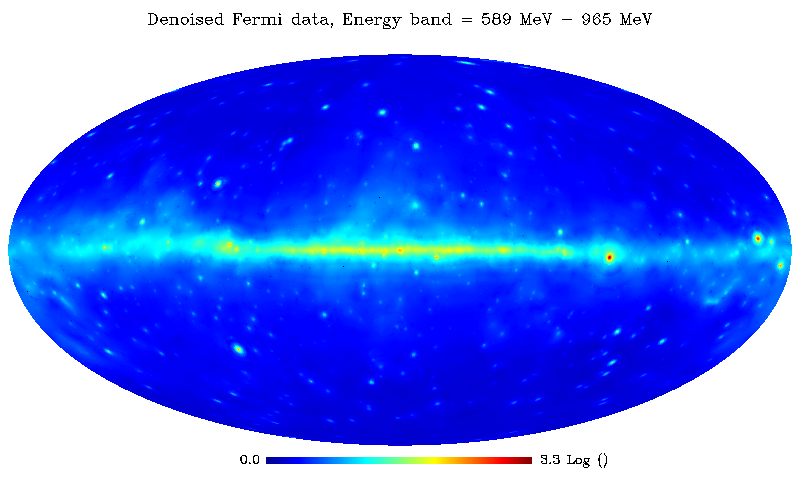
\includegraphics[width=3.8in]{sol5.png} \hfill
%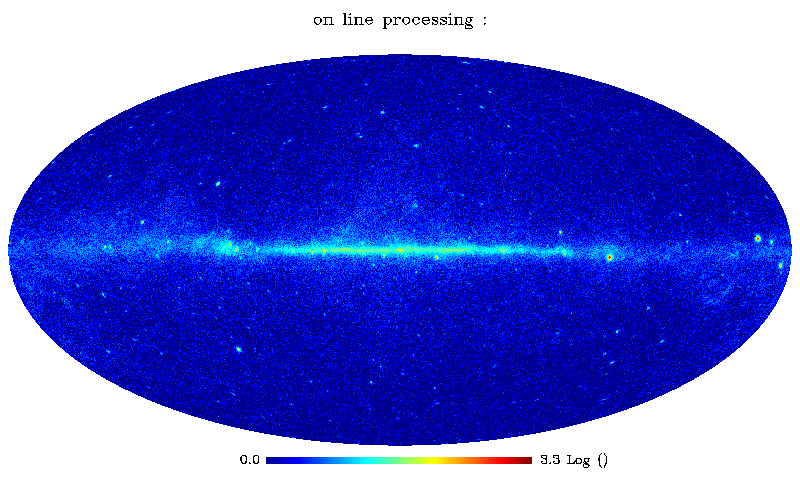
\includegraphics[width=3in]{data7.png} \hfill
%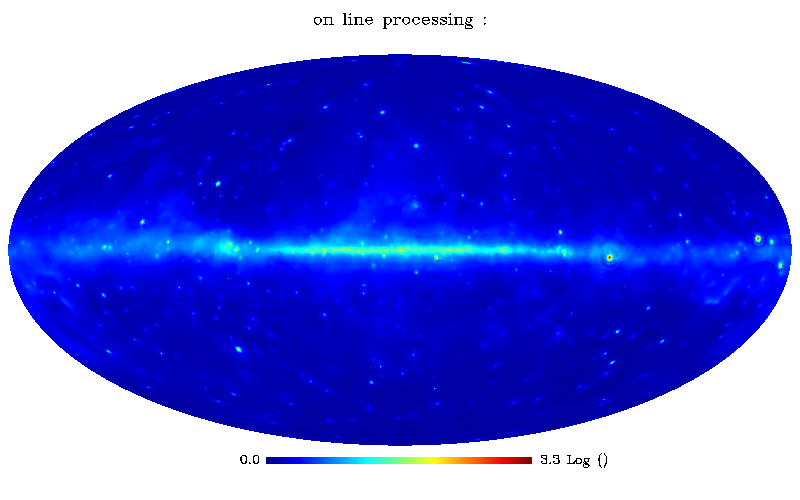
\includegraphics[width=3in]{sol7.png} \hfill
%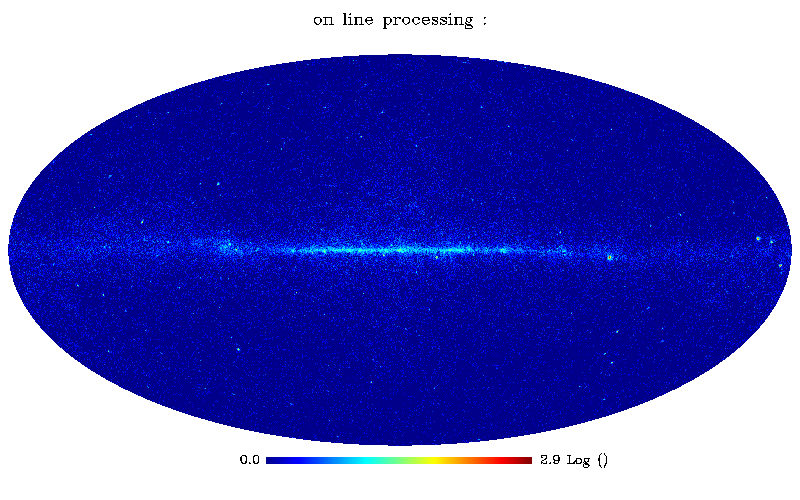
\includegraphics[width=2.9in]{data9.png} \hfill
%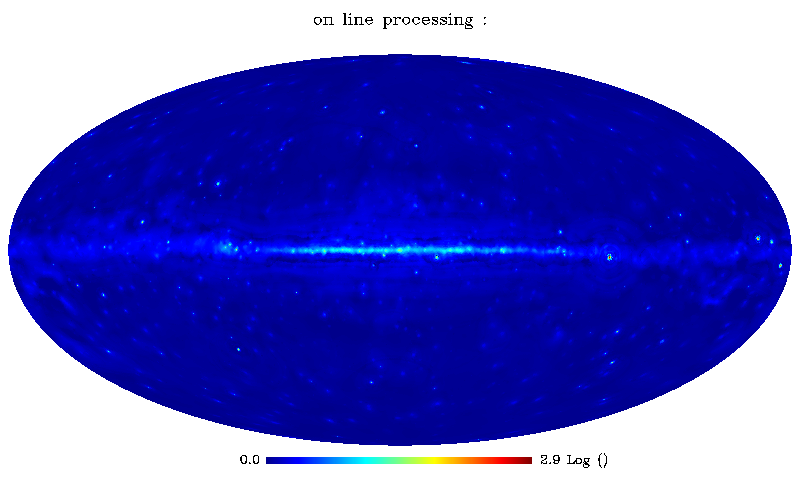
\includegraphics[width=2.9in]{sol9.png} \hfill
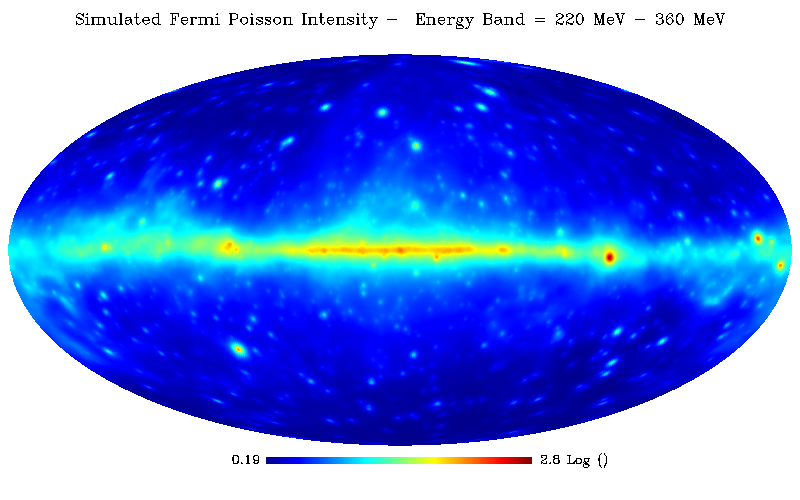
\includegraphics[width=3.8in]{plot_mc_intensityband3.png} \hfill
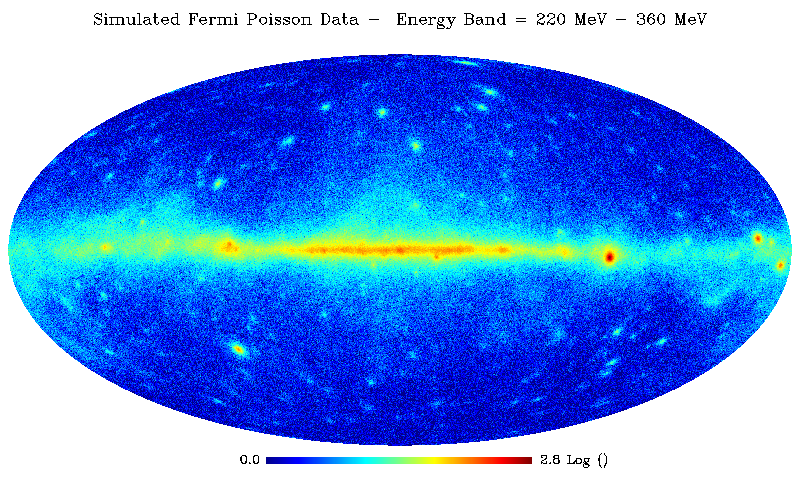
\includegraphics[width=3.8in]{plot_mc_simupoissonband3.png} \hfill
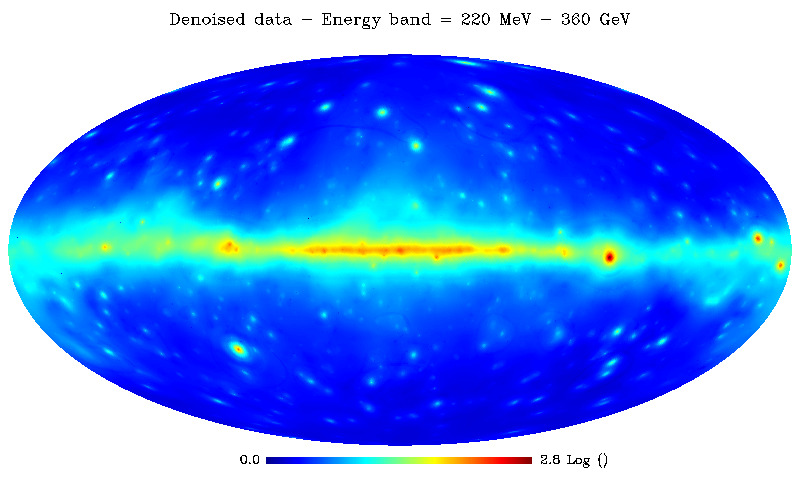
\includegraphics[width=3.8in]{plot_mc_simudenoisedband3.png} \hfill
\caption{Result of the multichannel Poisson denoising algorithm on simulated Fermi data on energy band 589 MeV - 965 MeV (\emph{Top:} Simulated intensity skymap. \emph{Middle:} Simulated noisy skymap. \emph{Bottom:} denoised skymap).
%Result of the multichannel Poisson denoising algorithm on simulated Fermi data on two different energy bands (Top : noisy skymap. Bottom : denoised skymap).
%Energy bands: 220 MeV - 360 MeV, 589 MeV - 965 MeV.
%Energy bands: 82 MeV - 134 MeV, 220 MeV - 360 MeV, 589 MeV - 965 MeV, 1.58 GeV - 2.59 GeV, 4.24 GeV - 69.5 GeV.
Pictures are in logarithmic scale.
}
\label{denoisingmulti2}
\end{center}
\end{figure}

%\begin{figure}
%\begin{center}
%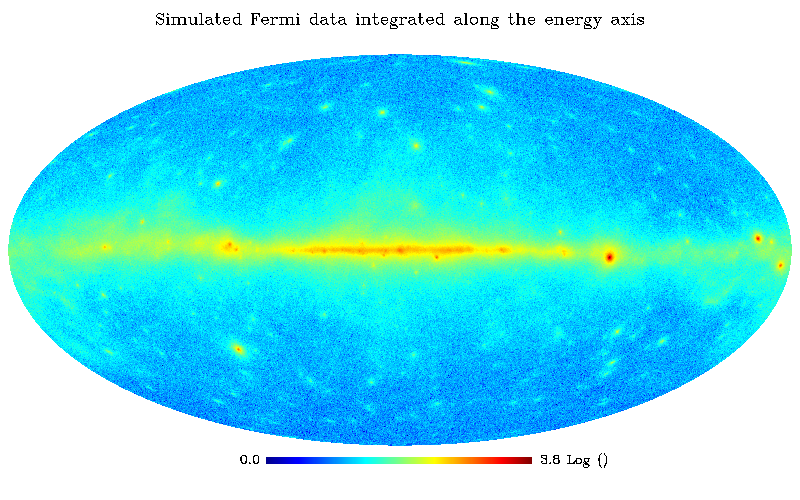
\includegraphics[width=3.9in]{datatot.png} \hfill
%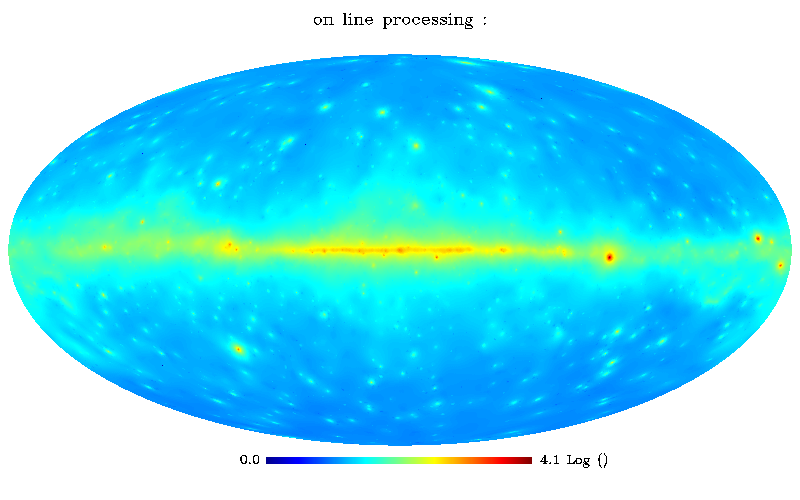
\includegraphics[width=3.9in]{datatotrec.png} \hfill
%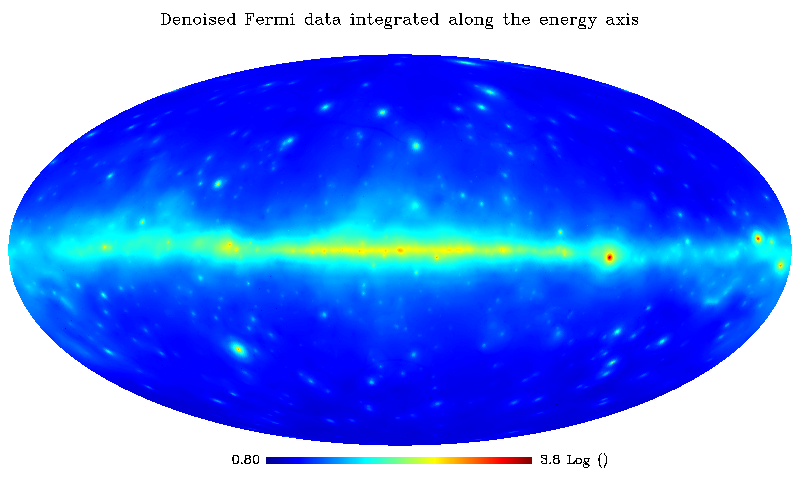
\includegraphics[width=3.9in]{solutiontot.png} \hfill
%\caption{Comparison of multichannel MS-VSTS denoising with monochannel MS-VSTS denoising. \emph{Top :} Simulated Fermi data integrated along the energy axis. \emph{Middle :} Simulated Fermi data integrated along the energy axis and denoised using monochannel MS-VSTS. \emph{Bottom :} Simulated Fermi data denoised with multichannel MS-VSTS and integrated along the energy axis.
%}
%\label{denoisingmulti2}
%\end{center}
%\end{figure}

\begin{figure}
\begin{center}
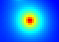
\includegraphics[width=0.5in]{plot_mc_sourceintensity.png}
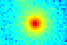
\includegraphics[width=0.5in]{plot_mc_sourcenoisy.png}
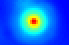
\includegraphics[width=0.5in]{plot_mc_sourcedenoised.png} \hfill
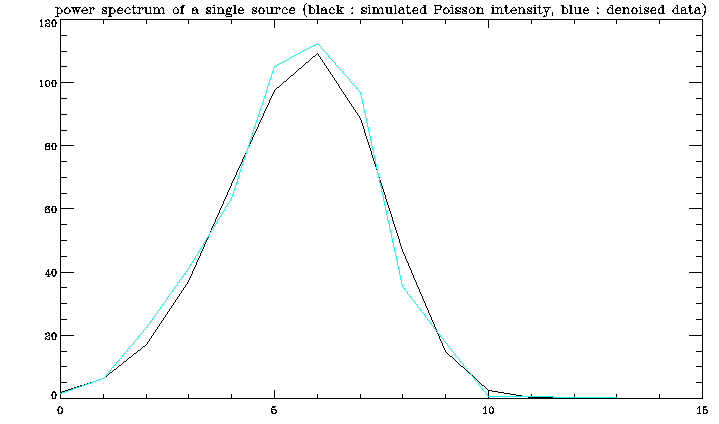
\includegraphics[width=5in]{plot_mc_spectrum.png}
\caption{Power spectrum of a single gamma ray point source recovered using the multichannel MS-VSTS denoising algorithm. \emph{Top:} Single gamma ray point source on simulated Fermi data integrated along the energy axis (\emph{Left:} Poisson Intensity. \emph{Middle:} Noisy data. \emph{Right:} Denoised data.) 
\emph{Bottom:} Power spectrum of the center of the denoised point source: intensity as a function of the energy band (\emph{Black:} Simulated Poisson intensity map. \emph{Blue:} Denoised map.)  (14 energy bands between 50 MeV and 50 GeV)%(7 energy bands between 50 MeV and 1.58 GeV).
}
\label{powspec}
\end{center}
\end{figure}


%vue d'une face Healpix
%spectre de puissance d'un pixel

\section{Multichannel Sparse Deconvolution for Spherical Poisson Data}

\subsection{Introduction}

Many problems in signal and image processing can be cast as inverting the linear system:

\begin{equation}
\label{linsyst}
y = \mathbf{H} x + \epsilon
\end{equation}

where $x \in \mathbb{R}^{N}$ is the data to recover, $y \in \mathbb{R}^{m}$ is the image of noisy observations, and $\epsilon$ is an additive noise with bounded variance. The unknown error can be either a stochastic measurement noise induced by the sensor, or a deterministic perturbation due for example to an imperfect signal model. $\mathbf{H} : \mathbb{R}^{N} \rightarrow \mathbb{R}^{m}$ is a bounded linear operator which is typically ill-behaved since it models an acquisition process that encounters loss of information. Eq. (\ref{linsyst}) is usually an ill-posed problem. This means that there is no unique and stable solution.


Our objective is to remove the effect of the instrument's PSF. In our case, $\mathbf{H}$ is the convolution by a blurring kernel (PSF) and $y$ lacks the high frequency content of $x$ and the problem above is a deconvolution problem.

In order to regularize such an inversion problem and reduce the space of candidate solutions, one has to add some prior knowledge on the typical structure of the original image $x$. This prior information account for the smoothness of the solution and can range from the uniform smoothness assumption to more complex knowledge of the geometrical structures of $x$.

%In the case of the LAT, the point spread function depends a lot on the energy, from about $3.5�$ at $100$ MeV to better than $0.1�$ at $10$ GeV and above.
In our LAT realistic simulations, the point spread function width depends a lot on the energy, from $6.9�$ at $50$ MeV to better than $0.1�$ at $10$ GeV and above. Figure~\ref{psfprofile} shows the normalized profiles of the PSF for different energy bands.

\begin{figure}
\begin{center}
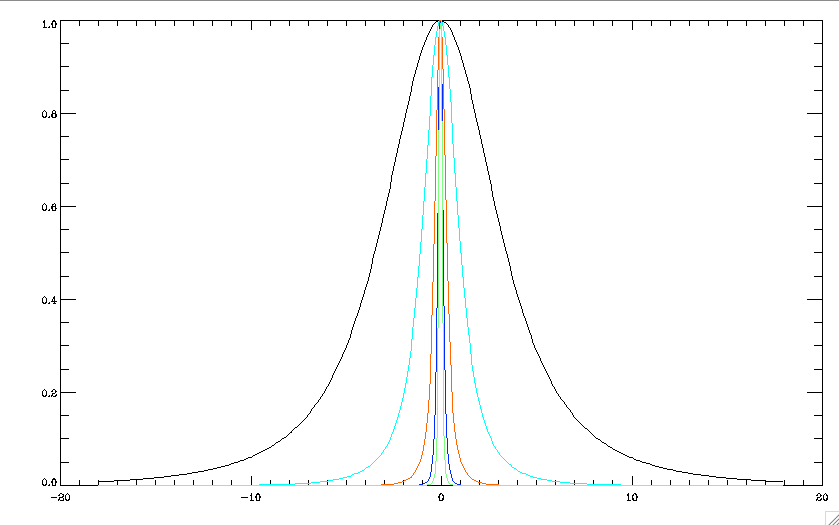
\includegraphics[width=6in]{psfprofile.png} \hfill
\caption{Normalized profile of the point spread function for different energy bands as a function of the angle in degree. \emph{Black:} $50$ MeV - $82$ MeV. \emph{Light Blue:} $220$ MeV - $360$ MeV. \emph{Orange:} $960$ MeV - $1.6$ GeV. \emph{Dark Blue:} $4.2$ GeV - $6.9$ GeV. \emph{Green:} $19$ GeV - $31$ GeV.}
\label{psfprofile}
\end{center}
\end{figure}


%exemples de PSF

\subsection{Monochannel Deconvolution}

For Poisson image deconvolution, several methods were proposed. Richardson-Lucy is certainly the most famous in astrophysics. In this paper, we propose a new regularized Richardon-Lucy algorithm for spherical Poisson data.

We denote $\mathbf{Y}$ the observed data, $\mathbf{H}$ the convolution kernel, and $\mathcal{N}(\mathbf{X})$ the additive noise. The deconvolution consists in estimating $\mathbf{X}$ so that:
\begin{equation}
\label{eq1}
\mathbf{Y}=\mathbf{H} \star \mathbf{X}+\mathcal{N}(\mathbf{ X})
\end{equation}
where $\star$ denotes the convolution product.

An iterative deconvolution scheme is given by Richardson-Lucy method. We start with $n=0$ and $\mathbf{X}^{(0)} = 1$ and we iterate:
\begin{equation}
\label{JVCmethod}
\mathbf{X}^{(n+1)} =P_+\Big[ \mathbf{X}^{(n)}  \Big( \mathbf{H}^{T} \ast \frac{\mathbf{Y}}{\mathbf{H} \ast \mathbf{X}^{(n)}} \Big)\Big]
\end{equation}
where $\mathbf{H}^{T}$ is the transpose of $\mathbf{H}$, and $P_+$ a positivity projection.


We define $\mathbf{R}^{(n)}$ the residual at iteration $n$:
\begin{equation}
\label{residual}
\mathbf{R}^{(n)} = \mathbf{Y}- (\mathbf{H} \ast \mathbf{X}^{(n)})
\end{equation}

By using the Isotropic Undecimated Wavelet Transform on the sphere (IUWT), $\mathbf{R}^{(n)}$ can be defined as the sum of its $J$ wavelet scales and the last smooth array, for a pixel $k$:
\begin{equation}
\label{waveletres}
\mathbf{R}^{(n)}[k] = a_J [k]  + \sum_{j=1}^{J} d_j [k]
\end{equation}
where $a_J$ denotes the last smoothed array, and $d_j$ denotes a wavelet scale.

The wavelet coefficients provide a mechanism to extract only the significant structures from the residual at each iteration. Normally, a large part of these residuals are statistically non-significant. The significant residual is then, for a pixel $k$:
\begin{equation}
\label{signifgauss}
\mathbf{\bar{R}}^{(n)}[k] = a_J [k]  + \sum_{j=1}^{J} \mathcal{M}(j,k) d_j [k]
\end{equation}
where $\mathcal{M}(j,k)$ is the multiresolution support.
The regularized iterative scheme becomes:
\begin{equation}
\label{regularizedJVC}
\mathbf{X}^{(n+1)} = P_+\Big[ \mathbf{X}^{(n)}  \Big( \mathbf{H}^{T} \ast \frac{\mathbf{H} \ast \mathbf{X}^{(n)} + \mathbf{\bar{R}}^{(n)}}{\mathbf{H} \ast \mathbf{X}^{(n)}} \Big)\Big]
\end{equation}




\subsection{Multichannel Deconvolution}

In this problem, the data can be viewed as a matrix $\mathbf{Y}=(Y_t)_t$, where, for each channel $t$, $Y_t = (y_{r,t})_{r}$ is the vector corresponding to the spherical data at channel $t$, where $r$ is the index corresponding to the pixel. Each channel is convolved by a known blurring kernel $\mathbf{ H}_t$ : $Y_t = \mathbf{ H}_t \star X_t + \mathcal{N}(X_t)$. 

We compute the spherical 2D-1D MS-VSTS transform, and the multiresolution support $\mathcal{M}_{j_1,j_2}[k_r,k_t]$ is obtained by hypothesis testings on coefficients.

We denote $\mathcal{H}$ the convolution by channel operator: $\mathcal{H} \mathbf{ X}$ means that each channel $X_t$ is convolved by the convolution kernel $\mathbf{ H}_t$. $\mathcal{H}^T \mathbf{ X}$ means that each channel $X_t$ is convolved by the transposed convolution kernel $\mathbf{ H}^T_t$. The regularized iterative scheme is then: \begin{equation}
\label{regularizedmcdeconv}
\mathbf{X}^{(n+1)} = P_+\Big[ \mathbf{X}^{(n)}  \Big( \mathcal{H}^{T} \frac{\mathcal{H} \mathbf{X}^{(n)} + \mathbf{\bar{R}}^{(n)}}{\mathcal{H} \mathbf{X}^{(n)}} \Big)\Big]
\end{equation}
with $\mathbf{\bar{R}}^{(n)}[k_r, k_t]$ the significant residual:
\begin{equation}
\begin{split}
\label{signifresmc}
\mathbf{\bar{R}}^{(n)}[k_r,k_t] = a_{J_1,J_2} [k_r,k_t] +  \sum_{j_1=1}^{J_1} \mathcal{M}_{j_1,J_2}[k_r,k_t] w_{j_1,J_2} [k_r,k_t]  \\ + \sum_{j_2=1}^{J_2}  \mathcal{M}_{J_1,j_2}[k_r,k_t] w_{J_1,j_2} [k_r,k_t] + \sum_{j_1=1}^{J_1} \sum_{j_2=1}^{J_2}  \mathcal{M}_{j_1,j_2}[k_r,k_t] w_{j_1,j_2} [k_r,k_t]
\end{split}
\end{equation}
where $\mathcal{M}_{j_1,j_2}$ is the multiresolution support.


%The reconstruction algorithm is:

%\begin{algorithm}[!h]
%%\caption{MS-VSTS + IUWT Denoising}
%\label{alg1}
%\begin{algorithmic}[1]
%\REQUIRE $\quad$ Input noisy data $\mathbf{Y}$, a low-pass filter $h$, multiresolution support $\mathcal{M}$ from the detection step, number of iterations $N_{\max}$ \\
%%\underline{\emph{\textbf{Detection}}} \\
%\STATE Initialize $\mathbf{X}^{(0)} = \mathcal{M} \mathcal{W} \mathbf{Y} = \mathcal{M}w_{Y}$,
%\FOR{$n=1$ to $N_{\max}$}
%\STATE $\tilde{d} = \mathcal{M}w_Y + (1-\mathcal{M})\mathcal{W}\mathcal{H}X^{(n-1)}$,
%\STATE $\mathbf{X}^{(n)} = P_{+}(\mathcal{H}^{T}\mathcal{R}\text{ST}_{\beta_n}[\tilde{d}])$,
%\STATE Update the step $\beta_n = (N_{\max} - n)/(N_{\max} - 1)$
%\ENDFOR

%\end{algorithmic}
%\end{algorithm}


\subsection{Experiments}

%The algorithm is applied on the 7 first energy bands of our simulated Fermi data set ($50 MeV$ to $1.58 GeV$).
The algorithm is applied on the 7 energy bands of our simulated Fermi data set ($50 MeV$ to $1.58 GeV$). Figures \ref{deconv1} to \ref{deconv4} show the result of the deconvolution on 4 energy bands.  %Figure \ref{deconv3} compares the result of the multichannel MS-VSTS deconvolution with the result of the multichannel MS-VSTS denoising on data integrated along the energy axis.
Figure \ref{deconv5} shows the effect of the MS-VSTS deconvolution algorithm on a single point source. The deconvolution gives a better spatial localisation for point sources. Figure \ref{deconv6} shows the effect of the MS-VSTS deconvolution algorithm on the galactic plan, where the effect of the deconvolution is particularly spectacular. Our MS-VSTS multichannel deconvolution algorithm manages to remove a large part of the PSF effect.

\begin{figure}
\begin{center}
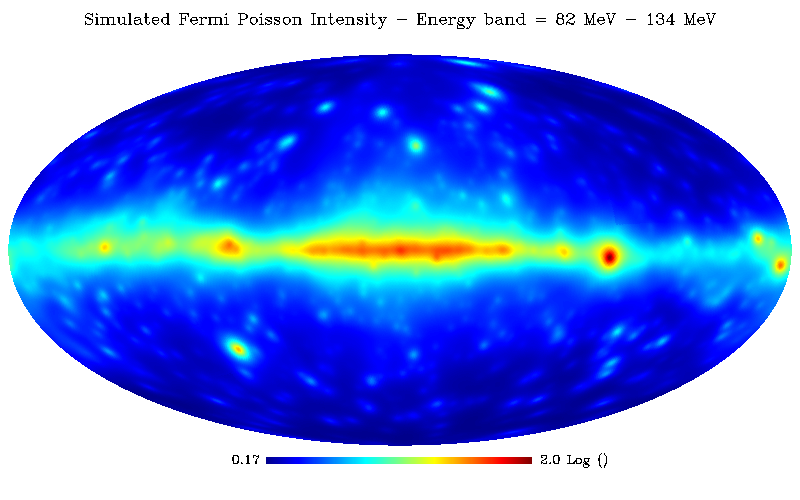
\includegraphics[width=3.8in]{plot_mc_intensityband1.png} \hfill
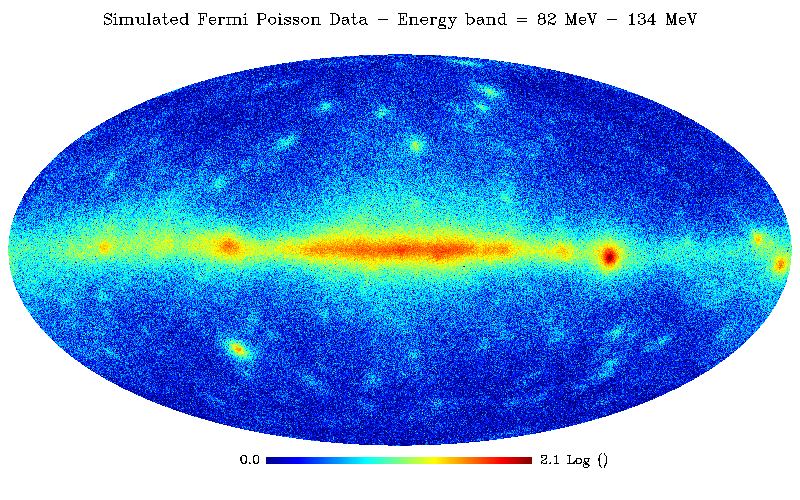
\includegraphics[width=3.8in]{plot_mc_simupoissonband1.png} \hfill
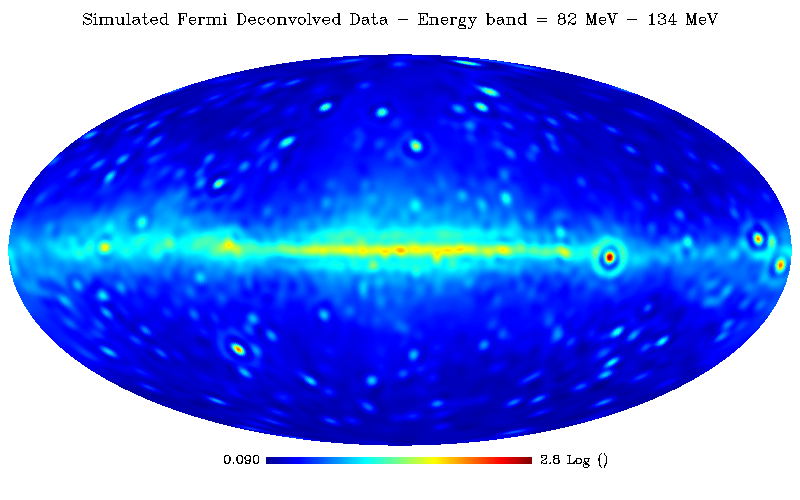
\includegraphics[width=3.8in]{plot_mc_simudeconvband1.png}
\caption{Result of the multichannel deconvolution algorithm on different energy bands (\emph{Top:} Simulated Intensity skymap. \emph{Middle:} noisy skymap. \emph{Bottom:} deconvolved skymap).
%Energy bands : 50 MeV - 82 MeV, 82 MeV - 134 MeV, 134 MeV - 220 MeV, 220 MeV - 360 MeV.
Energy band : 82 MeV - 134 MeV.
Pictures are in logarithmic scale.
}
\label{deconv1}
\end{center}
\end{figure}

\begin{figure}
\begin{center}
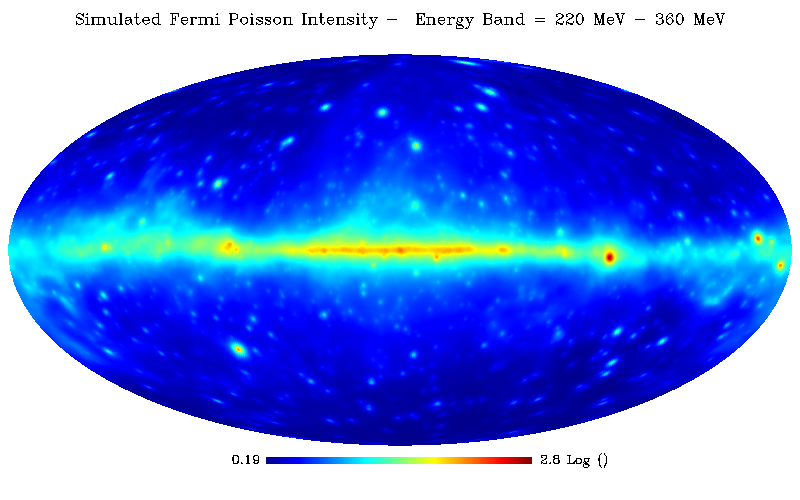
\includegraphics[width=3.8in]{plot_mc_intensityband3.png} \hfill
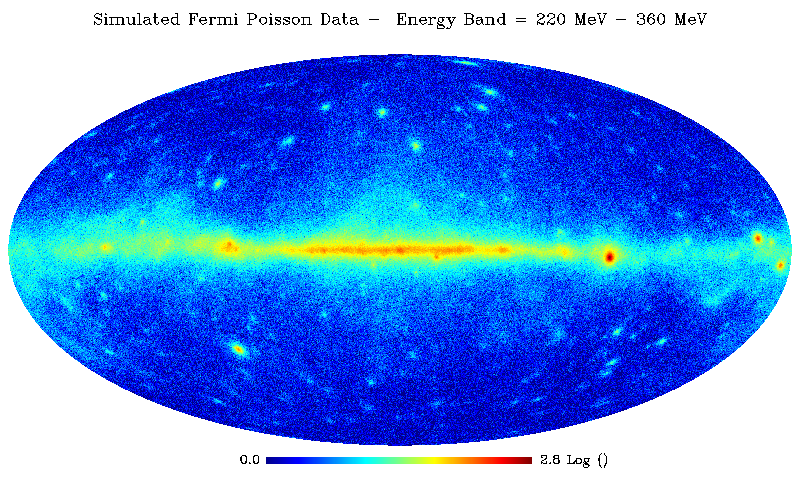
\includegraphics[width=3.8in]{plot_mc_simupoissonband3.png} \hfill
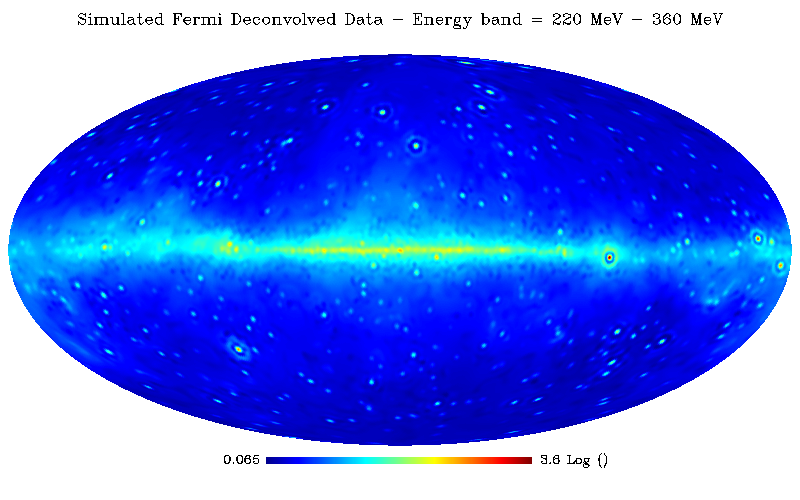
\includegraphics[width=3.8in]{plot_mc_simudeconvband3.png}
\caption{Result of the multichannel deconvolution algorithm on different energy bands (\emph{Top:} Simulated Intensity skymap. \emph{Middle:} noisy skymap. \emph{Bottom:} deconvolved skymap).
%Energy bands : 50 MeV - 82 MeV, 82 MeV - 134 MeV, 134 MeV - 220 MeV, 220 MeV - 360 MeV.
Energy band : 220 MeV - 360 MeV.
Pictures are in logarithmic scale.
}
\label{deconv2}
\end{center}
\end{figure}

\begin{figure}
\begin{center}
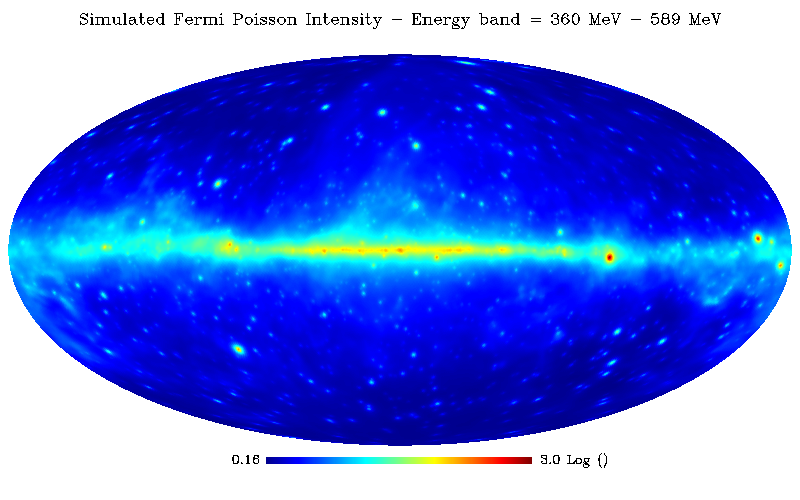
\includegraphics[width=3.8in]{plot_mc_intensityband4.png} \hfill
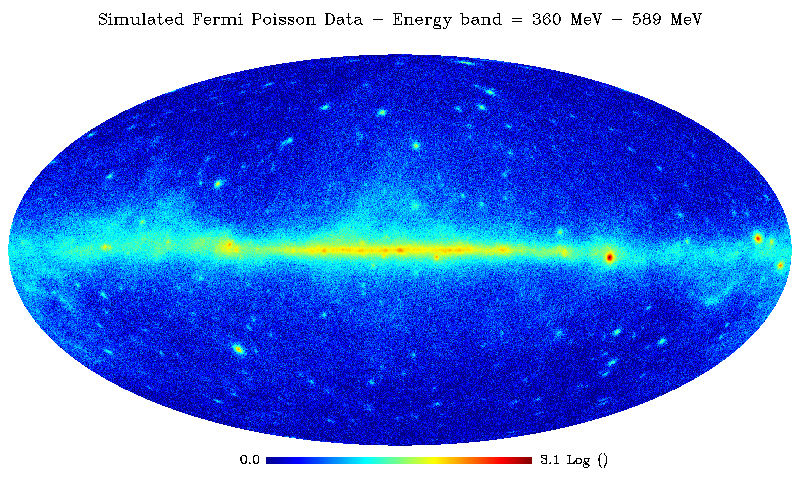
\includegraphics[width=3.8in]{plot_mc_simupoissonband4.png} \hfill
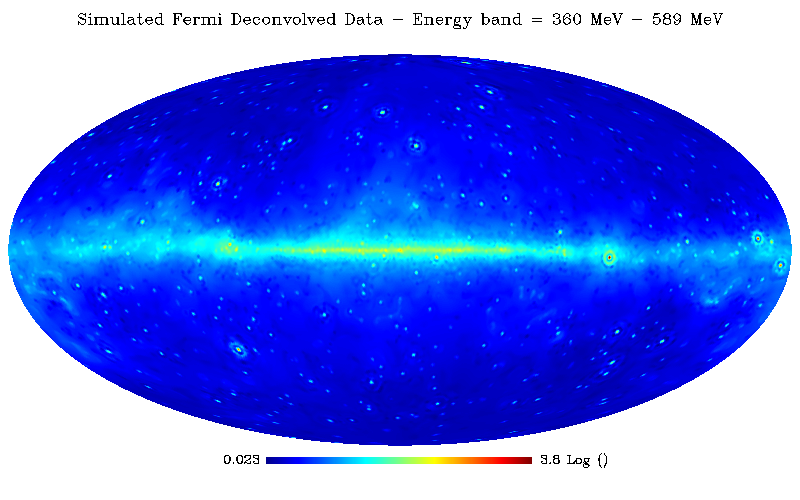
\includegraphics[width=3.8in]{plot_mc_simudeconvband4.png}
\caption{Result of the multichannel deconvolution algorithm on different energy bands (\emph{Top:} Simulated Intensity skymap. \emph{Middle:} noisy skymap. \emph{Bottom:} deconvolved skymap).
%Energy bands : 50 MeV - 82 MeV, 82 MeV - 134 MeV, 134 MeV - 220 MeV, 220 MeV - 360 MeV.
Energy band : 360 MeV - 589 MeV.
Pictures are in logarithmic scale.
}
\label{deconv3}
\end{center}
\end{figure}

\begin{figure}
\begin{center}
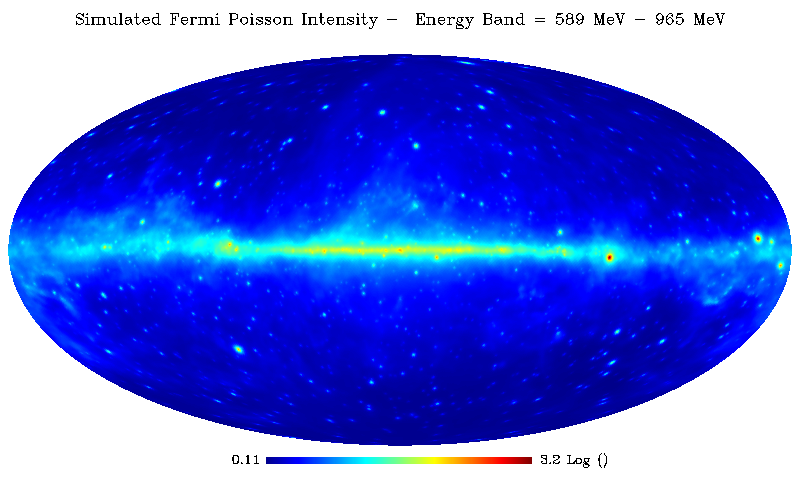
\includegraphics[width=3.8in]{plot_mc_intensityband5.png} \hfill
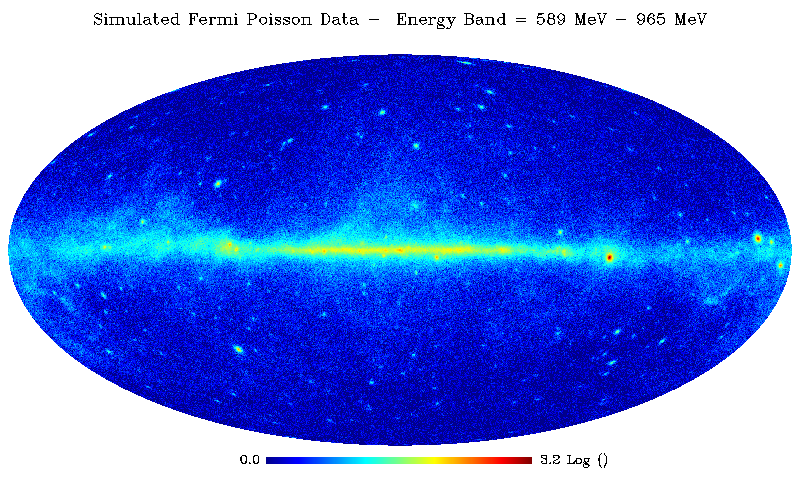
\includegraphics[width=3.8in]{plot_mc_simupoissonband5.png} \hfill
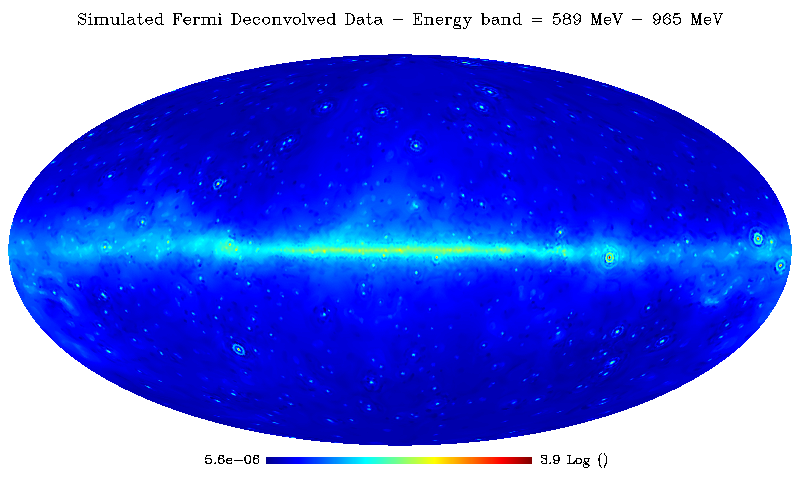
\includegraphics[width=3.8in]{plot_mc_simudeconvband5.png}
\caption{Result of the multichannel deconvolution algorithm on different energy bands (\emph{Top:} Simulated Intensity skymap. \emph{Middle:} noisy skymap. \emph{Bottom:} deconvolved skymap).
%Energy bands : 50 MeV - 82 MeV, 82 MeV - 134 MeV, 134 MeV - 220 MeV, 220 MeV - 360 MeV.
Energy band : 589 MeV - 965 MeV.
Pictures are in logarithmic scale.
}
\label{deconv4}
\end{center}
\end{figure}


%\begin{figure}
%\begin{center}
%%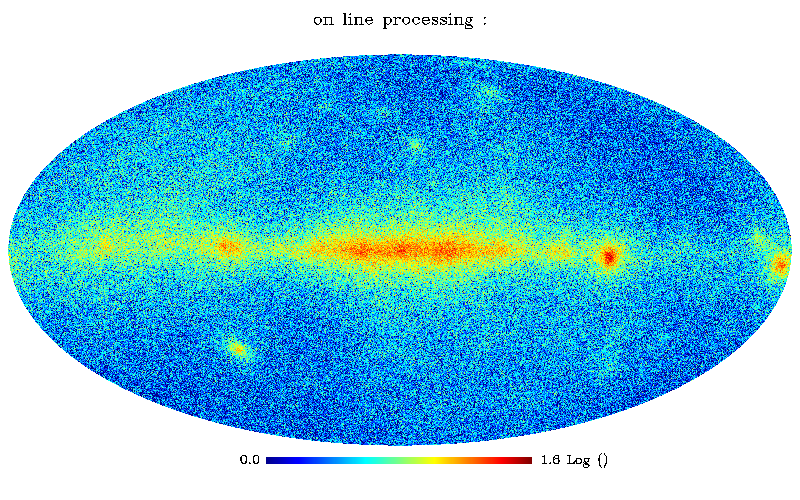
\includegraphics[width=2.9in]{data0.png} \hfill
%%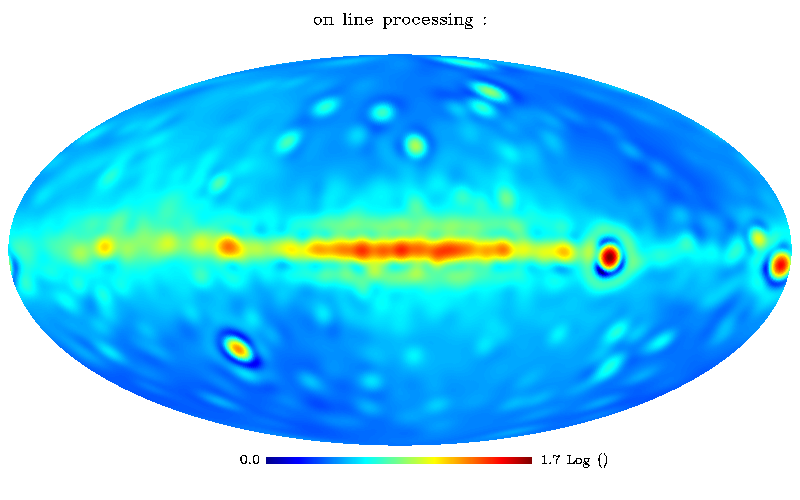
\includegraphics[width=2.9in]{donnees0deconv.png} \hfill
%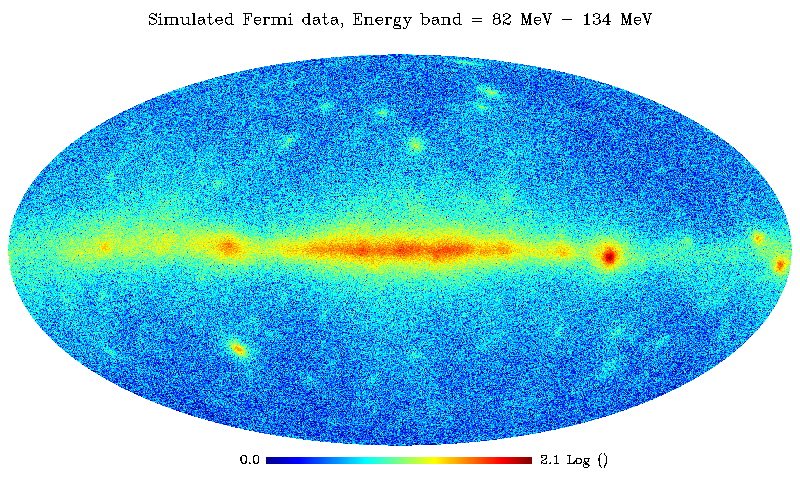
\includegraphics[width=3.8in]{data1.png} \hfill
%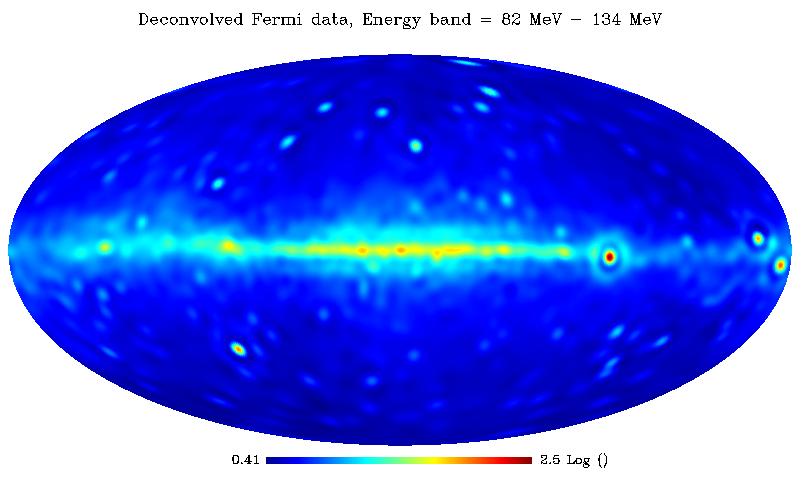
\includegraphics[width=3.8in]{data1deconv.png} \hfill
%%\includegraphics[width=2.9in]{data2.png} \hfill
%%\includegraphics[width=2.9in]{donnees2deconv.png} \hfill
%\includegraphics[width=3.8in]{data3.png} \hfill
%\includegraphics[width=3.8in]{data3deconv.png} \hfill
%\caption{Result of the multichannel deconvolution algorithm on different energy bands (First : noisy skymap. Second : deconvolved skymap).
%%Energy bands : 50 MeV - 82 MeV, 82 MeV - 134 MeV, 134 MeV - 220 MeV, 220 MeV - 360 MeV.
%Energy bands : 82 MeV - 134 MeV, 220 MeV - 360 MeV.
%Pictures are in logarithmic scale.
%}
%\label{deconv1}
%\end{center}
%\end{figure}


%\begin{figure}
%\begin{center}
%\includegraphics[width=3.8in]{data4.png} \hfill
%\includegraphics[width=3.8in]{data4deconv.png} \hfill
%%\includegraphics[width=2.9in]{data5.png} \hfill
%%\includegraphics[width=2.9in]{donnees5deconv.png} \hfill
%\includegraphics[width=3.8in]{data5.png} \hfill
%\includegraphics[width=3.8in]{data5deconv.png} \hfill
%\caption{Result of the multichannel deconvolution algorithm on different energy bands (First : noisy skymap. Second : deconvolved skymap).
%%Energy bands : 360 MeV - 589 MeV, 589 MeV - 965 MeV, 965 MeV - 1.58 GeV.
%Energy bands : 360 MeV - 589 MeV, 589 MeV - 965 MeV.
%Pictures are in logarithmic scale.
%}
%\label{deconv2}
%\end{center}
%\end{figure}
%
%\begin{figure}
%\begin{center}
%\includegraphics[width=5in]{sourceprofile.png}
%\caption{Profile of a single point source on the 6th energy band. In blue, the skymap is denoised using a monochannel MS-VSTS+Wavelets. In black, the data is deconvolved using multichannel MS-VSTS.
%}
%\label{deconvmono3}
%\end{center}
%\end{figure}



%\begin{figure}
%\begin{center}
%\includegraphics[width=3.8in]{datatot.png} \hfill
%\includegraphics[width=3.8in]{solutiontot.png} \hfill
%%\includegraphics[width=2.9in]{data5.png} \hfill
%%\includegraphics[width=2.9in]{donnees5deconv.png} \hfill
%\includegraphics[width=3.8in]{donneesdeconvtot.png} \hfill
%\caption{\emph{Top:} Simulated Fermi data integrated along the energy axis. \emph{Middle:} Simulated Fermi data denoised with multichannel MS-VSTS and integrated along the energy axis. \emph{Bottom:} Fermi data deconvolved with multichannel MS-VSTS and integrated along the energy axis. 
%%Energy bands : 360 MeV - 589 MeV, 589 MeV - 965 MeV, 965 MeV - 1.58 GeV.
%Pictures are in logarithmic scale.
%}
%\label{deconv3}
%\end{center}
%\end{figure}


%\begin{figure}
%\begin{center}
%\includegraphics[width=1.5in]{sourcenoisy.png}
%\includegraphics[width=1.5in]{sourcedenoised.png}
%\includegraphics[width=1.5in]{sourcedeconv.png} \hfill
%\includegraphics[width=5in]{profilesource.png}
%\caption{Comparison of the effect of the multichannel denoising algorithm with the multichannel deconvolution algorithm on a single gamma ray point source on data integrated along the energy axis. \emph{Top:} Single gamma ray point source on simulated Fermi data integrated along the energy axis (\emph{Left:} Noisy data. \emph{Middle:} Denoised data. \emph{Right:} Deconvolved data.) 
%\emph{Bottom:} Profile of the point source . In blue, the denoised source. In black, the deconvolved source.
%}
%\label{deconv4}
%\end{center}
%\end{figure}

\begin{figure}
\begin{center}
%\includegraphics[width=1.5in]{plot_mc_source_intensity.png}
%\includegraphics[width=1.5in]{plot_mc_source_noisy.png}
%\includegraphics[width=1.5in]{plot_mc_source_deconv.png} \hfill
\includegraphics{plot_mc_source_intensity.png}
\includegraphics{plot_mc_source_noisy.png}
\includegraphics{plot_mc_source_deconv.png} \hfill
\includegraphics[width=5in]{plot_mc_source_profile.png}
\caption{Effect of the multichannel deconvolution algorithm on a single gamma ray point source. \emph{Top:} Single gamma ray point source on simulated Fermi data (Energy band: 360 MeV - 589 MeV) (\emph{Left:} Intensity. \emph{Middle:} Noisy data. \emph{Right:} Deconvolved data.) 
\emph{Bottom:} Profile of the point source. In blue, the source from intensity map. In black, the deconvolved source.
}
\label{deconv5}
\end{center}
\end{figure}

%\begin{figure}
%\begin{center}
%\includegraphics[width=2.9in]{datatotnoisyface.png} \hfill
%\includegraphics[width=2.9in]{datatotdenoisedface.png} \hfill
%\includegraphics[width=2.9in]{datatotdeconvface.png}
%\caption{View on a single HEALPix face. Comparison of the multichannel denoising algorithm with the multichannel deconvolution algorithm on the galactic plan. \emph{Top Left:} Simulated Fermi data integrated along the energy axis. \emph{Top Right:} Simulated Fermi data denoised with multichannel MS-VSTS and integrated along the energy axis. \emph{Bottom:} Fermi data deconvolved with multichannel MS-VSTS and integrated along the energy axis. 
%%Energy bands : 360 MeV - 589 MeV, 589 MeV - 965 MeV, 965 MeV - 1.58 GeV.
%Pictures are in logarithmic scale.
%}
%\label{deconvtot}
%\end{center}
%\end{figure}

\begin{figure}
\begin{center}
\includegraphics[width=2.9in]{plot_mc_plane_intensity.png} \hfill
\includegraphics[width=2.9in]{plot_mc_plane_noisy.png} \hfill
\includegraphics[width=2.9in]{plot_mc_plane_deconv.png}
\caption{View on a single HEALPix face. Result of the deconvolution algorithm on the galactic plan. \emph{Top Left:} Simulated Fermi Poisson intensity. \emph{Top Right:} Simulated Fermi noisy data. \emph{Bottom:} Fermi data deconvolved with multichannel MS-VSTS. 
Energy band: 360 MeV - 589 MeV.
Pictures are in logarithmic scale.
}
\label{deconv6}
\end{center}
\end{figure}